Until now has been discussed pipeline execution on a single node. Since now will be exposed how to delivery the execution of the pipeline in cluster mode.\newline
In Background chapter explains how Spark works and the possibility that offers Spark to distribute computation in cluster. Microsoft Azure offers a solution, \textit{HDInsight}, which provides a pre-configured environment ready to execute Spark in cluster mode. The inconvenient is the pricing, which is the double of a normal VM without the HDInsight provisioning. Instead of invest moneys in HDInsight, is better spending them in further hardware resources.\newline
Rather than spending resources in HDInsight, the choice is to provision VMs "by hand". To delivery this provisioning has been chosen Docker Swarm.

\section{VMs Provisioning with Docker Swarm}
GATK 4.0 Spark tools give the opportunity to run them in cluster mode. But they expect to read input files or reference genome in HDFS. So Docker should be able to provide both services (Spark over HDFS). The solution Docker Swarm, as exposed in Background chapter, offers the opportunity to deploy a service over a cluster in order to have Docker Containers distributed in different nodes, able to communicate with each other. Through \textbf{Docker Stack} has been possible distributing the required services on cluster. It is based on a \textit{docker-compose} file, just like services in local machine; with some differences, Docker Stack allows to distribute services over a Swarm.\newline
\textit{\href{https://www.big-data-europe.eu/}{Big Data Europe}} offers a solution that allows to achieve this task; indeed they provide in Docker Hub the Docker Images necessary to deploy containers over a Swarm.\newline
According to Spark and HDFS architectures exposed in Background chapter, the required actors for this cluster are \textbf{Namenode}, \textbf{Datanode}, \textbf{Spark Mater} and \textbf{Spark Worker}, illustrated in Figure \ref{NGS_services_swarm}. First of all it is necessary to create a Swarm: the first node will be \textbf{Swarm Manager}, following nodes that will join the \textit{swarm} are \textbf{Swarm Worker}. After that is possible to deploy the stack.
\begin{figure}[h] 
\begin{center}
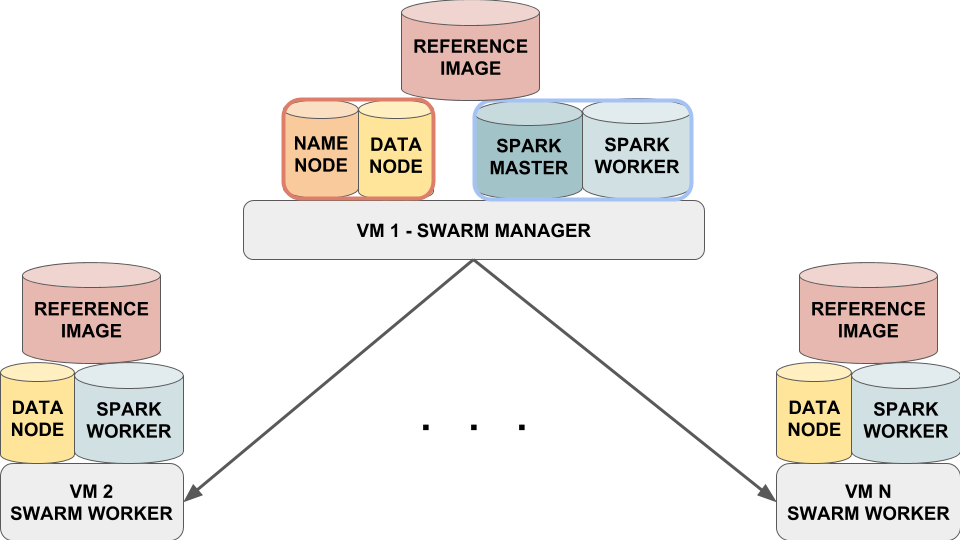
\includegraphics[scale=0.45]{figure/stack_spark_hdfs.png}
\end{center}
\caption{Services distribution of the NGS Pipeline over a cluster ~\label{NGS_services_swarm}}
\end{figure}
\\[1\baselineskip]
As described in Background chapter, both HDFS and Spark have a Master-Slave architecture, where Spark Master and Namenode are masters, Datanode and Spark Worker are slaves. In a consistent manner, the masters have been deployed in the Swarm Manager, specifying an only replica in docker-compose file. Slaves may be deployed in global mode, distributing for each slave a replica in each node which is part of the Swarm. These containers will be able to communicate through a declared Overlay Network.\newline
It is important to expose these ports, in order to get relative benefits:
\begin{itemize}
  \item 4040 (Spark Master): provides a monitoring service of the running job, through a graphic user interface; it is very useful for debugging and understanding the job status.
  \item 8080 (Spark Master): gives an overview of the Spark-cluster, useful to understand if there is any communication issue and all Spark Workers correctly joined the cluster. 
  \item 7077 (Spark Master): used to launch Spark jobs in cluster mode, indeed at the moment of executing \textit{spark-submit} script and specifying Spark parameters, the Spark Master will be expressed in this way: \textit{--spark-master spark://SPARK-MASTER-HOST:7077}
  \item 8081 (Spark Worker): gives information about the Spark Worker; indeed when executing in cluster-mode, Spark stack-trace is really poor of information. Here is possible to observe the usual stack trace printed in local-mode, or even in the Spark Worker container at \textit{/spark/work/[0-9]+/stderr}
  \item 50070 (Namenode): a graphic interface that allows to navigate the HDFS and other operations.
\end{itemize}
But the environment is not ready yet. Indeed just like in local execution mode, it is necessary to provide to the pipeline reference genome files, input samples, annotation databases, GATK 4.0 \& 3.8, Picard ecc.\newline
So has been used the Spark Master Docker image provided by Big Data Europe as a starting point, for then adding the required dependencies. Indeed the Spark Master Dockerfile will clone the GATK GitHub repository for then installing it, obtaining in this way GATK 4.0. With COPY command have been put GATK 3.8 and Picard jars inside the container. Eventually have been added environment variables and Spark logs service. The image of this container is available in my \href{https://hub.docker.com/r/vzzarr/spark-master/}{Docker Hub repository} .\newline
In docker-compose files have been specified \textbf{volumes}, a feature that allows to Docker containers inside a stack to access the host machine's file system. In this way the Spark Master is able to access to input samples and all annotation databases.\newline
The reference genome in cluster mode must be treated in particular manner. As exposed in a \href{https://github.com/broadinstitute/gatk/issues/3186}{GATK GitHub issue}, the GATK Spark tools require for .2bit reference genome in HDFS and the reference image distributed for each Spark Worker file system. This means that is necessary to distribute this file in each node of the cluster, so that the Spark Worker is able to access it. This explains the Reference Image container in Figure \ref{NGS_services_swarm}, indeed has been used a Docker container with global deployment mode, to globally distribute to all the Swarm nodes the reference genome image. Through the volumes is then possible to give to Spark Worker the access to Reference Image container file system and access in this way the reference genome image file. This approach has been preferred since that in this way is easy to change reference genome. If the user would like to use another reference genome, he only needs to create a container with the relative reference image inside.

\section{Cluster-mode Execution}
Now that the environment has been provisioned, is possible to run the service. An overview of the work-flow has been illustrated in Figure \ref{distributed_pipeline}, where the entire process can be divided in 4 steps:
\begin{enumerate}
  \item \textbf{FastqToSam} - as previously anticipated in section \textit{Sparkifying not-Spark tools}, for this moment it is not possible to use in distributed mode these tools, only in local mode. Indeed as shown in the picture, only the Spark Master container is accountable to execute this tool, without distributing the work-load to Spark-Worker containers in the various Swarm nodes. Anyway this processing gets benefit from the number of cores of the host machine, when there are more sample files to convert in uBAM.
  \item \textbf{Load files to HDFS} - when the uBAM files produced  by FastqToSam are available, is possible to distribute them in HDFS. Not only the uBAM files, but even reference files and known sites files will be loaded in HDFS. In particular the script will use the Namenode container as interface, in order to use HDFS commands and distribute the specified files over Datanodes.
  \item \textbf{GATK Spark Tools} - these tools, when executed in distributed mode, require some input files from HDFS, that are the files distributed in the previous step. In particular are:
  \begin{enumerate}
  	\item \textit{BwaAndMarkDuplicatesPipelineSpark}: this tool requires the uBAM file and reference genome .2bit file in HDFS as previously mentioned, and reference genome in local file system. This last requirement has been achieved through Reference Image container as previously explained. Moreover in this \href{https://github.com/broadinstitute/gatk/issues/3186}{GATK GitHub issue} has been discussed about an important parameter, \textit{--bam-partition-size}. Without this parameter, the relative default value is set to 0, with the result of getting stuck during the execution of this tool. Setting this parameter to 4000000, as expressed in that topic, the execution proceeds and reaches the completion. From tool documentation: \textit{maximum number of bytes to read from a file into each partition of reads. Setting this higher will result in fewer partitions. Note that this will not be equal to the size of the partition in memory. Defaults to 0, which uses the default split size (determined by the Hadoop input format, typically the size of one HDFS block).  Default value: 0.}
    \item \textit{BQSRPipelineSpark}: here is requested the output file of the previous tool in HDFS (not a problem, since is possible to write it directly in HDFS), the reference .2bit file in HDFS (the same for BwaAndMarkDuplicatesPipelineSpark) and known sites in HDFS, which have already been loaded previously in HDFS. When trying to execute it in cluster mode, I faced with a \href{https://github.com/broadinstitute/gatk/issues/4376}{Spark performance regression}, that has been patched in following GATK update in version 4.0.2.0.
    \item \textit{HaplotypeCallerSpark}: similar to BQSRPipelineSpark, is requested the output generated by the previous tool in HDFS and reference genome .2bit file in HDFS. The Spark performance regression was even here, but the patch made by GATK resolved this issue too.
  \end{enumerate}
  \item \textbf{\textit{Sparkified} Tools} - just like for FastqToSam, even other Sparkified Tools (already described in Pipeline chapter) may be executed only in local mode, taking the input file from normal file system. So before of executing this tools is necessary to move the output generated by HaplotypeCallerSpark in HDFS to normal file system. Even here tools get benefit from the number of cores of the host machine.
\end{enumerate}


\begin{figure}[h] 
\begin{center}
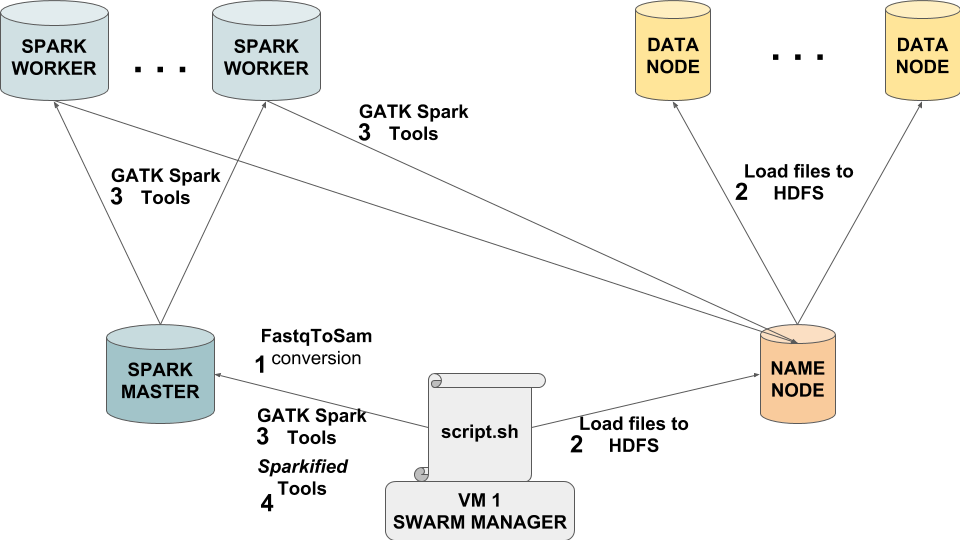
\includegraphics[scale=0.45]{figure/distributed_pipeline.png}
\end{center}
\caption{Pipeline work-flow in Distributed mode ~\label{distributed_pipeline}}
\end{figure}





















